%!TEX root = ../bomberchamp.tex


To capture the spatial relations between objects on the field, we use a 2D convolutional neural network. This network takes a matrix $X\in\mathbb{R}^{w\times h \times c} $ as input, where $w$ and $h$ are width and height respectively and $c$ is the number of channels. In the case of bomberman, we have $w=h=17$. For the arena and objects in the game world we give each its own channel (Figure \ref{fig:input-channels}):

\begin{tabular}{l p{0.7\linewidth}}
Walls & $\in\left\{0,1\right\}$ \\
Crates & $\in\left\{0,1\right\}$ \\
Self & $\in\left\{0,1,2\right\}$, this channel gets omitted when we later center the inputs. \\
Others & $\in\left\{0,1,2\right\}$\\
Bombs & $\in\left[0, 1\right]$ \\
Explosions & $\in\left\{0,1\right\}$ \\
Coins& $\in\left\{0,1\right\}$ \\
\end{tabular}

In the channels \emph{self} for the player agent and \emph{others} for the opponents,
$$X_{x,y}|_{c=self/others}=\begin{cases}
2 & \text{player with bomb,} \\
1 & \text{player without bomb,} \\
0 & \text{otherwise.}
\end{cases}
$$

There is no differentiation between the different opponents, since the state only consists of the current time step.
For bombs $(x, y, t)$, $t$ being the time left until the bomb explodes, we calculate $$X_{x, y}|_{c=\text{bombs}} = 1 - \frac{t}{\mathrm{bombtimer}+1} \;\;\forall (x, y, t) \in \text{bombs}$$ with $$X_{x, y}|_{c=\text{bombs}}=0 \;\;\forall (x, y, t\geq0) \notin \text{bombs}.$$
So with $\text{bombtimer}=4$, if $X_{x, y}|_{c=\text{bombs}} = 0.2$, the bomb has just been planted, and if $X_{x, y}|_{c=\text{bombs}} = 1$, the bomb will explode this turn.
While an explosion is active for two turns, this includes when the bomb timer hits zero, so the explosion is only visible to agents during one turn.


\begin{figure}
  \centering
  % Store largest image in a box
  \savebox{\largestimage}{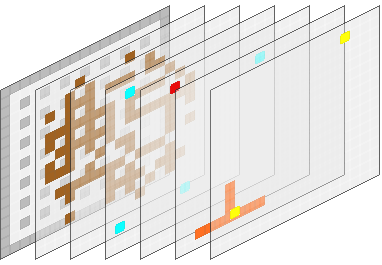
\includegraphics[height=.22\textheight]{images/X_channel-layers.png}}%
  \begin{subfigure}[b]{0.6\textwidth}
    \centering
    \usebox{\largestimage}
    \caption{Visualization of the separate channels}
  \end{subfigure}
  \quad
  \begin{subfigure}[b]{0.36\textwidth}
    \centering
    % Adjust vertical height of smaller image
    \raisebox{\dimexpr.5\ht\largestimage-.5\height}{%
      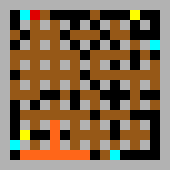
\includegraphics[height=.18\textheight]{images/X_channel-full.png}}
    \caption{All channels combined}
  \end{subfigure}
  \caption{Input channels (from left to right): walls (gray), crates (brown), self (turquoise), other players (turquoise), bombs (red), explosions (orange), coins (yellow)}
  \label{fig:input-channels}
\end{figure}

The matrix $X$ is sparse in all but two channels, but this feature space captures the spatial correlations well.

A very important part of the input is the position of the agent itself. If the player position is simply transformed into a channel, it is reduced to one of many variables and it can be difficult to pick up the importance of this specific variable. So to simplify learning for our agent, the agent was centered in the feature space, so that it stays at a fixed position while the environment (coins, crates, other agents) move around it. To implement this, the size of the feature space is increased to $(2w-1, 2h-1, c)$ size and the agent placed in the middle of the new board.
